\documentclass[journal,a4paper]{article}
\usepackage{fullpage}
\usepackage{float}
\usepackage[T1]{fontenc}

%\usepackage{color}
\usepackage{parskip}
\usepackage{enumerate}
\usepackage{xcolor}
\usepackage{amsmath}
\usepackage{graphicx}
\usepackage{listings}


\begin{document}
\onecolumn

\title{COMP333: Assignment 2}
\author{James Ridey\\
44805632}
\maketitle
%
%\lstdefinestyle{customc}{
%  belowcaptionskip=1\baselineskip,
%  breaklines=true,
%  frame=L,
%  xleftmargin=\parindent,
%  language=,
%  showstringspaces=false,
%  basicstyle=\footnotesize\ttfamily,
%  keywordstyle=\bfseries\color{green!40!black},
%  commentstyle=\itshape\color{purple!40!black},
%  identifierstyle=\color{blue},
%  stringstyle=\color{orange},
%}

\definecolor{pblue}{rgb}{0.13,0.13,1}
\definecolor{pgreen}{rgb}{0,0.5,0}
\definecolor{pred}{rgb}{0.9,0,0}
\definecolor{pgrey}{rgb}{0.46,0.45,0.48}

\lstset{language=Java,
  showspaces=false,
  showtabs=false,
  tabsize=4,
  breaklines=true,
  showstringspaces=false,
  breakatwhitespace=true,
  commentstyle=\color{pgreen},
  keywordstyle=\color{pblue},
  stringstyle=\color{pred},
  basicstyle=\ttfamily,
  moredelim=[il][\textcolor{pgrey}]{$ $},
  moredelim=[is][\textcolor{pgrey}]{\%\%}{\%\%}
}

\pagenumbering{gobble}
\hyphenation{water question questions maximum}
\section*{Question 1}
\begin{enumerate}[(a)]
	\item What this invariant is saying is that for every item in the queue, it is at least 1 distance away from the head of the queue. This holds true for eveyr iteration of the BFS algorithm because of a few reasons, the first is that nodes are added onto the end of the queue, the second is that we never visit the same node twice and the third reason is that BFS always expands equally in every direction. For these three reasons nodes in the queue will always be in ascending distance.
	\item For every visited node, the distance is made of a combination of the cells that are reachable (Fact 1) and the node that is the closest to them. BFS expands equally in all directions so every visited nodes distance is simply the closest previous node that used to be in the queue.
	\item 
\end{enumerate}

\section*{Question 2}
\begin{enumerate}[(a)]
	\item For each loop of divideBasic we are subtracting b from a. For a worst case scenario this means we have something like 99999 / 1. Expressing this in the form a and b means we get $10^{L(a)}-1$ and $10^{L(b)-1}$. 

Given we are subtracting each loop iteration this means we have $\frac{10^{L(a)}-1}{10^{L(b)-1}}$ operations. And so the Big-Oh of divideBasic is 
	\begin{align*}
		&= \frac{10^{L(a)}-1}{10^{L(b)-1}} \\
		&= 10^{L(a)-(L(b)-1)} - 1 \\
		&= O(10^{L(a)-L(b)+1})
	\end{align*}
	\item To figure out the time complexity for divide we first need to figure out how big divisorShifted gets, the first while loop basically keeps multiplying $b$ by 10 until it is larger than $a$, this can be expressed as so.
	\begin{align*}
		b\cdot 10^x &> a \\
		10^x &> \frac{a}{b} \\
		x &> log_{10}(\frac{a}{b}) \\
	\end{align*}
	The first thing to note is that the $log_{10}(a) \approx L(a)$. So this means
	\begin{align*}
		&= log_{10}(\frac{a}{b}) \\
		&= log_{10}(a)-log_{10}(b) \\
		&= L(a) - L(b) \\
	\end{align*}
	Then the next thing to note is the main while loop runs through the size of the divisorShifted plus 1 because $x$ only corresponds to how many zero's we added to divisorShifted and the loop is removing a zero each time. This means the main while loop is doing $L(a)-L(b)+1$ iterations.
	
	Lastly every loop iteration we are doing a subtraction on remainder, this subtraction is inside a while loop but this while loop only executes 10 times at most because it is basically doing digit subtraction and the largest and smallest digit we can have is 9 and 1. The time complexity for a subtraction is $L(a)$, multiplying this by the amount of times the outer main while loop executes we get $L(a)(L(a)-L(b)+1)$
\\\\\
	(We can effectively ignore the addition on the quotient because it is not operating on $a$ or $b$. This is the same as if I was getting the time complexity for summing an array, we can ignore the constant operations that are happening inside the loop because they aren't operating on the array.)
	
	\item The best way to understand this question is with some graphs
	\\\\
	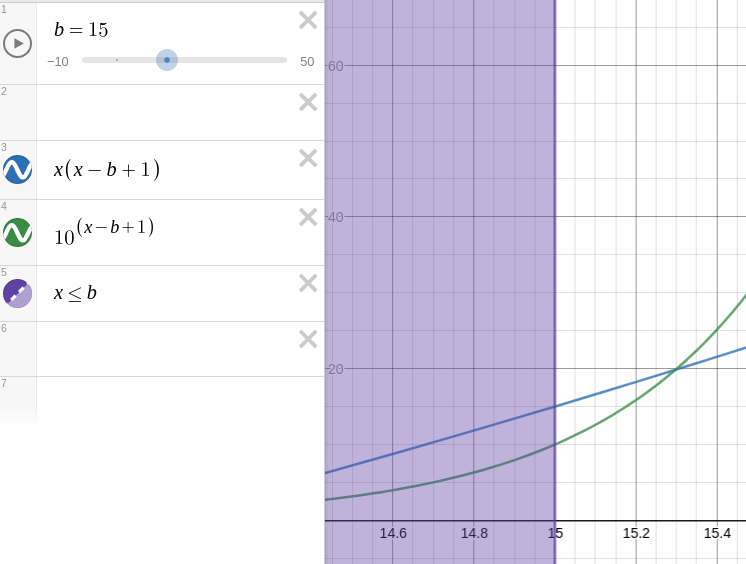
\includegraphics[scale=2]{divide-complexity-1} \\
	In this graph we have the green line as divideBasic and the blue line as divide, we have a L(b) of 15, L(a) being set as the x variable and y being O(n). From this graph we can see initially divideBasic wins out if the length of both numbers are the same, however it quickly loses out as the length of a grows.
	\\\\
	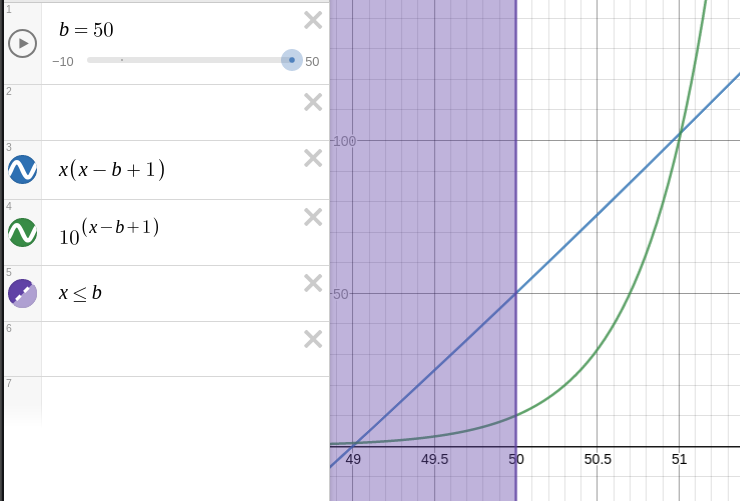
\includegraphics[scale=2]{divide-complexity-2} \\
	As b increases, divideBasic is the faster variant as long as a and b are the same length.
	\\\\
	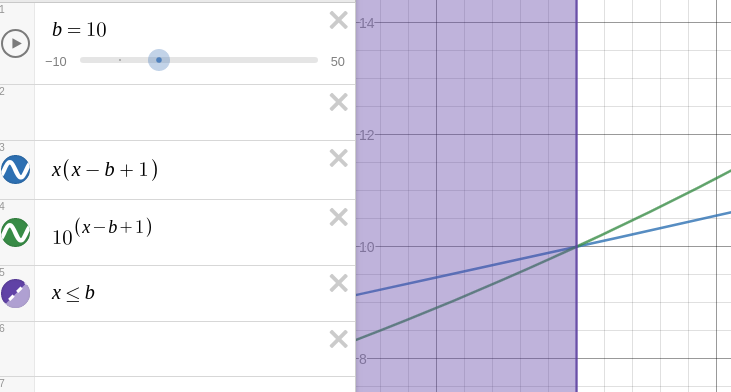
\includegraphics[scale=0.5]{divide-complexity-3} \\
	The exception to this rule is with lengths of b less than 10, this this case divide is always faster than divideBasic.
	\\\\
	In conclusion, divideBasic is only ever faster than divide when the lengths of the numbers are the same, for every other case divide wins out exponentially.	
\end{enumerate}

\section*{Question 3}
\begin{enumerate}[(a)]
	\item TODO \begin{lstlisting}
	public static int[] egcd(int a, int b) {
		int x0 = 1;
		int x1 = 0;
		int y0 = 0;
		int y1 = 1;

		while (b != 0) {
			int qdiv = a / b;
			int qmod = a % b;

			a = b;
			b = qmod;

			int t = x1;
			x1 = x0-x1*qdiv;
			x0 = t;

			t = y1;
			y1 = y0-y1*qdiv;
			y0 = t;
		}

		int[] result = new int[3];
		result[0] = a;
		result[1] = x0;
		result[2] = y0;
		return result;
	}
	\end{lstlisting}

	\item TODO \begin{lstlisting}
	public static int minv(int a, int n) {
		int[] egcd = egcd(a, n);
		return Math.floorMod(egcd[1],n);
	}
	\end{lstlisting}
	
	\item TODO \begin{lstlisting}
	public static int cra(int p, int q, int a, int b) {
		int sum = a*q*minv(q,p) +
		  	      b*p*minv(p,q);

		return Math.floorMod(sum, p*q);
	}
	\end{lstlisting}
\end{enumerate}

\section*{Question 4}
\begin{enumerate}[(a)]
	\item Loop invariant: $a^{b_0} \equiv ra^b\ (mod\ n)$, where $b_0$ is the original $b$ value.
	
		  TOFIX: For this algorithm it runs until b is zero and for every iteration of the loop we divide b by 2. So this loop runs at least $log_2(b)$ times. During the loop operation we do 2 multiplications and 2 divisions, while 1 of the multiplications and 1 of the divisions is behind an if statement in the worse case scenario (Big-Oh), if a number was simply a 1 bit repeated it would always trigger the if statement.
		  
		  So for the worse case scenario we have
		  \begin{align*}
		  	&= log_2(b)(2mul + 2div) \\
		  	&= log_2(b)(2(L(a)L(b)) + 2(L(a)(L(a)-L(b)+1))) \\
		  	&= log_2(b)(2(L(a)(L(a)+1))) \\
		  \end{align*}
	\item \begin{lstlisting}
	public static BigInt modexpv2(BigInt a, BigInt b, BigInt n) {
		//Euler thereom
		//a^b mod m = a^(b mod phi(m)) mod m

		//phi(p) where p is prime is p-1
		return modexp(a, b.divide(n.subtract(ONE))[1], n);
	}
	\end{lstlisting}
	
	\item \begin{lstlisting}
	TODO:
	public static int modexpv3(int a, int b, int p, int q) {
		BigInt ab = new BigInt(String.valueOf(a));
		BigInt bb = new BigInt(String.valueOf(b));
		BigInt pb = new BigInt(String.valueOf(p));
		BigInt qb = new BigInt(String.valueOf(q));

		BigInt cd1b = modexpv2(ab,bb,pb);
		BigInt cd2b = modexpv2(ab,bb,qb);

		int cd1 = Integer.valueOf(cd1b.toString());
		int cd2 = Integer.valueOf(cd2b.toString());
		int pinv = minv(p,q);

		return Math.floorMod(cd1 + p * pinv * (cd2 - cd1), p*q);
	}
	\end{lstlisting}
\end{enumerate}

\section*{Question 5}
TOFIX: For the time complexity of Karatsuba we first need to find out how deep the tree of the recursion will go. Using what we understand of the algorithm and how it effectively splits the numbers in half each time. The depth of the tree is $log_2(max(L(a),L(b)))$.

Then for every node of the recursion we do the following
\begin{enumerate}[(a)]
	\item Call Karatsuba another three times
	\item 2 additions
	\item 2 multiplications
	\item 2 subtractions
	\item 2 lessThanOrEqual's
	\item 2 modpows - (similar time complexity to modexp)	
\end{enumerate}

This effectively means we have the time complexity of
\begin{align*}
	&= log_2(max(L(a),L(b)))\cdot \left( 3(2add+2mul+2sub+2less+2modpow) \right) \\
	&= log_2(max(L(a),L(b)))\cdot \left( 3(2add+2mul+2sub+2less+2modpow) \right) \\
\end{align*}

Generally karatsuba is less efficient for numbers of small length due to the amount of extra steps that needs to be taken specifically the splitting of strings which can be done through string manipulation or through division and modulo operations. However once we start getting to digits that are hundreds of digits long then Karatsuba can be significantly faster than the classical method.

\section*{Question 6}
\begin{lstlisting}[language=Java]
static BigInt a = new BigInt("1140671485");
static BigInt c = new BigInt("128201163");
static BigInt m = bigpow(TWO, new BigInt("24"));
static BigInt rand = new BigInt(String.valueOf((int)(Math.random()*(Integer.MAX_VALUE-1))));

public static BigInt randombigint(BigInt low, BigInt high) {
	rand = a.multiply(rand).add(c).divide(m)[1];

	BigInt r = karatsuba(rand, high.subtract(low).add(ONE)).divide(m)[0];

	return low.add(r);
}
\end{lstlisting}

Firstly lets start off with how I generate random BigInt's, this is an example of a linear congruential generator which takes on the form $X_{n+1} = (aX_n+c)\ mod\ m$ and where a,c,m are carefully chosen to appear to make random numbers. Another part of this algorithm is it has to be initialised with a seed, the starting $X_n$ for this I've used Math.random() to generate an initial seed which is then passed into BigInt, this is done on the program startup.

The next part of the function is quite simply mapping the range 0 to m to low to high using this system, $low + rand(high-low+1)$. The interesting thing to note is that since BigInt doesn't support fractionals, I'm multiply the random number by $high-low+1$ before dividing it.

\begin{lstlisting}
public static boolean millerrabin(BigInt n, int s) {
	if (n.isEqual(TWO) || n.isEqual(THREE)) return true;
	if (n.divide(TWO)[1].isEqual(ZERO) || (n.lessOrEqual(TWO) && !n.isEqual(TWO))) return false;

	int s2 = 0;
	BigInt nMinusOne = n.subtract(ONE);
	BigInt d = nMinusOne;
	while (true) {
		BigInt[] divmod = d.divide(TWO);
		if (!divmod[1].isEqual(ZERO)) break;
		d = divmod[0];
		s2++;
	}

	witnessLoop:
	for (; s >= 0; s--) {
		BigInt a = randombigint(TWO,nMinusOne);
		BigInt x = modexp(a,d,n);
		if (x.isEqual(ONE) || (x.isEqual(nMinusOne))) continue;

		for (int i = s2-1; i >= 0; i--) {
			x = modexp(x,TWO,n);
			if (x.isEqual(ONE)) return false;
			if (x.isEqual(nMinusOne)) continue witnessLoop;
		}
		return false;
	}

	return true;
}

public static BigInt randomprime(int l, int s) {
	List<Character> evens = Arrays.asList('0','2','4','6','8');

    while (true) {
		BigInt low = new BigInt("1"+(String.join("", Collections.nCopies(l-1, "0"))));
	    BigInt high = new BigInt(String.join("", Collections.nCopies(l, "9")));
		BigInt random = randombigint(low, high);

		//Check if the last digit is even and if so replace it so it is now odd
	    String randomString = random.toString();
	    int n = randomString.length()-1;
		char lastChar = randomString.charAt(n);
        if (evens.contains(lastChar)) {
            lastChar += 1;
            random = new BigInt(randomString.substring(0,n)+lastChar);
        }

	    if (millerrabin(random, s)) return random;
	}
}
\end{lstlisting}
The next part of this question is the MillerRabin algorithm and the randomprime function. The MillerRabin algorithm is an algorithm for determining if a given number is prime within a certain probability, it returns false if it is definitely not a prime and true if it hasn't found a reason for it not to be prime.

The randomprime algorithm is quite simple, you call it and it returns a randomprime of length $l$, the workings of it are also quite simple, it simply loops creating random BigInt's, changes the BigInt to odd if the generated BigInt is even and then uses the MillerRabin test to see if it is prime to the probability set by $s$.

\section*{Question 7}
Most of the RSA program is input parsing and checking to make sure that the input being passed is correct. Cutting out that, I've pasted below the meat of the program.
\begin{lstlisting}[language=Java]
public static void encrypt(Scanner scanner) {
	...
	
	BigInt p = randomprime(length, 32);
	BigInt q = randomprime(length, 32);
	BigInt n = p.multiply(q); //TODO: Replace with karatsuba
	BigInt totient = p.subtract(ONE).multiply(q.subtract(ONE));

	BigInt publicKey;
	while (true) {
		publicKey = randomprime(totient.toString().length(), 32);

		int a = Integer.valueOf(totient.toString());
		int b = Integer.valueOf(publicKey.toString());

		if (publicKey.lessOrEqual(totient) && egcd(a,b)[0] == 1) break;
	}

	int a = Integer.valueOf(publicKey.toString());
	int b = Integer.valueOf(totient.toString());
	int privateKey = minv(a,b);

	System.out.println("Public key: " + publicKey);
	System.out.println("Private key: " + privateKey);
	System.out.println("Modulus: " + n);

	System.out.print("Data to encrypt: ");
	s = scanner.nextLine();
	for (char c : s.toCharArray()) {
		int pki = Integer.valueOf(publicKey.toString());
		int pi = Integer.valueOf(p.toString());
		int qi = Integer.valueOf(q.toString());

		int zz = modexpv3(pi, qi, (int)c, pki);
		System.out.print(zz+" ");
	}
	System.out.println('\n');
}

public static void decrypt(Scanner scanner) {
	...
	
	System.out.print("Private key: ");
	String s = scanner.nextLine();
	BigInt privateKey = new BigInt(s);

	System.out.print("Modulus: ");
	s = scanner.nextLine();
	BigInt n = new BigInt(s);

	System.out.print("Data: ");
	s = scanner.nextLine();
	for (String v : s.split(" ")) {
		BigInt d = new BigInt(v);
		int c = Integer.parseInt(modexp(d, privateKey, n).toString());
		System.out.print((char)c);
	}
	System.out.println('\n');
}
\end{lstlisting}

For encryption, we need to generate a private key, a public key and a modulus. To do this we follow these steps
\begin{enumerate}
	\itemsep0em
	\item Pick a random prime (p) and another random prime (q)
	\item Pick the public key to be a prime between 0 and the totient of p times q which for primes is $(p-1)\cdot (q-1)$.
	\item Check that the totient and the generated public key have a GCD of 1 and if not regenerate the public key.
	\item The private key is generated using the modular inverse of the public key and the totient.
	\item For every chuck in the data to be encrypted, take the modular exponent of the chunk, the public key and the modulus ($n = p\cdot q$)
\end{enumerate}

Decryption is a simpler process, for every chuck in the data to be decrypted, take the modular exponent of the chunk, the private key and the modulus and then concatenate all the results together making sure to convert the int's back to char's.

\end{document}
